\chapter{Experiments\label{cha:chapter4}}
This chapter details the experiments conducted in the context of this thesis.
We evaluate the proposed methods on three image classification datasets:
MNIST \cite{lecun2010mnist},
CIFAR-10 \cite{krizhevsky2009learning},
and Imagenette \cite{DBLP:journals/information/HowardG20}, which is a subset of 10 easily classified classes from the ImageNet dataset.
First, we provide an overview of the experimental setup.
We then present the results of the gradient ratio thresholding method, as detailed in Section \ref{sec:nestedquantizationlayer},
followed by the results of the custom loss terms discussed in Section \ref{sec:customloss}.

% ------------------------------------------------------------
% ----------------------- Setup ----------------------- 
% ------------------------------------------------------------

\section{Experimental Setup}
\label{sec:setup}
\textbf{Software and Hardware Setup.} As briefly mentioned in Section \ref{sec:nestedquantizationlayer},
our custom methods are implemented in TensorFlow.
Specifically, we used TensorFlow version 2.11.0, running on Python 3.10.14. 
All experiments are conducted on a server equipped with two NVIDIA A40 GPUs, 
each with 48 GB of memory, running on CUDA 11.4 and driver version 470.256.02.
\\
\\
\textbf{Experiment Networks.} 
For simplicity and tractability, we define custom networks for each dataset.
For MNIST, we use a small network consisting of two dense layers, 
each adjusted to incorporate nested quantization layers for both weights and biases. 
For CIFAR-10, we use a convolutional network with three blocks of convolutional layers, 
each adjusted to incorporate nested quantization layers for both kernels and biases.
These are followed by two dense layers.
The Imagenette model is a ResNet-inspired architecture,
featuring an initial quantized convolutional block followed by four stages of residual blocks. 
Each residual block incorporates the adjusted convolutional layers with nested quantization 
for both kernels and biases. For the experimentation with custom loss terms, 
we use equivalent networks without the nested quantization layer logic.
\\
\\
\textbf{Baseline Hyperparameters and Initialization.} Using the hyperparameters described in Table \ref{tab:hyperparameters}, 
each network optimizes its parameters using the Adam optimizer and the sparse categorical cross-entropy loss function. 
Weights and biases are initialized with random normal values, 
while scale factors are initialized with very small constant values for all cases. 
Scale factors are constrained to be positive and non-zero to avoid numerical issues during division. 
An example implementation for reproducing these networks is available at the following GitHub Gist: INSERT LINK

\begin{table}[h!]
    \centering
    \caption{Network Settings for Different Datasets}
    \label{tab:hyperparameters}
    \begin{tabular}{l|c|c|c}
    \hline
    \textbf{Hyperparameter}     & \textbf{MNIST} & \textbf{CIFAR-10} & \textbf{Imagenette} \\ \hline
    Learning Rate               & 0.0001          & 0.0001             & 0.001              \\ \hline
    Batch Size                  & 32             & 128                & 64                 \\ \hline
    Epochs                      & 100             & 100               & 100                \\ \hline
    Seed for Reproducibility    & 42             & 42                & 42                 \\ \hline
    \end{tabular}
\end{table}


% ------------------------------------------------------------
% ----------------------- Pareto stuff ----------------------- 
% ------------------------------------------------------------

\section{Optimal Thresholds for Nested Quantization Layers}
\label{sec:paretofronts}
For the nested quantization layer method, we evaluate the results across different thresholds \( \lambda \)
for both dense and convolutional layers. The first subsection presents results for fully connected layers trained on MNIST,
while the second subsection focuses on convolutional layers trained on CIFAR-10 and Imagenette.

\subsection{Fully Connected Layers}
\label{subsec:paretofrontsdense}
As mentioned earlier, we use a small network with two dense layers trained on the MNIST dataset. 
These two dense layers consist of weight matrices \( W_1 \) and \( W_2 \),
along with bias vectors \( b_1 \) and \( b_2 \).
We examine three scenarios:
applying the scale factor rowwise, 
column-wise, and as a single scalar for the entire weight matrix.
For all scenarios, a single scalar scale factor is used for each bias. 
The configurations are summarized in Table \ref{tab:scalefactorgranularitydense}.

\begin{table}[h!]
  \centering
  \caption{Scale Factor Granularity}
  \label{tab:scalefactorgranularitydense}
  \begin{tabular}{l|c|c|c|c}
  \hline
  \textbf{Granularity}        & \( W_1 \) \( (784 \times 128) \)       & \( b_1 \) \( (128,) \)        & \( W_2 \) \( (128 \times 10) \)     & \( b_2 \) \( (10,) \) \\ \hline
  Rowwise scaler              & \( s \) \( (784, ) \)                 & \( s \) \( (,) \)             & \( s \) \( (128, ) \)              & \( s \) \( (,) \)     \\ \hline
  Columnwise scaler           & \( s \) \( (,128) \)                  & \( s \) \( (,) \)             & \( s \) \( (,10) \)                & \( s \) \( (,) \)     \\ \hline
  Scalar scaler               & \( s \) \( (,) \)                     & \( s \) \( (,) \)             & \( s \) \( (,) \)                  & \( s \) \( (,) \)     \\ \hline
  \end{tabular}
  \vspace{0.5em}
  \caption*{\footnotesize Note: \( (,) \) represents a scalar value — scalars technically have no dimensions.}
\end{table}

\noindent The experiments have shown that the optimal quantization is observed for a penalthy threshold of 
\( \lambda = 1e-10 \) across all three scenarios.
This conclusion is based on Pareto front plots in Figure \ref{fig:pareto-mnist-unique-vals-accuracy},
which illustrate the trade-off between accuracy loss and quantization.
Specifically, we observe that, for all scenarios, 
the number of unique integer values after quantization, 
aggregated across all parameters of the two dense layers, reaches its lowest point at \( \lambda = 1e-10 \)
without significantly degrading the accuracy.
\\
\\
As an example, the actual integer values after quantization for the rowwise scenario is 
depicted in Figure \ref{fig:quantization_results_1e-10_dense} for all four parameters separately.
While the total number of unique values is only \( 10 \), the range spans from \( -5 \) to \( 5 \).
This means that \( 4 \) bits are sufficient to represent the quantized values in the resulting layers, 
as \( \lceil \log_2(11) \rceil = 4 \), covering all 10 unique values within the range. 
This can even be further reduced using Huffman coding, 
considering the concentration of values around 0 in the distributions.
\\
\begin{figure}[h!]
  \centering
  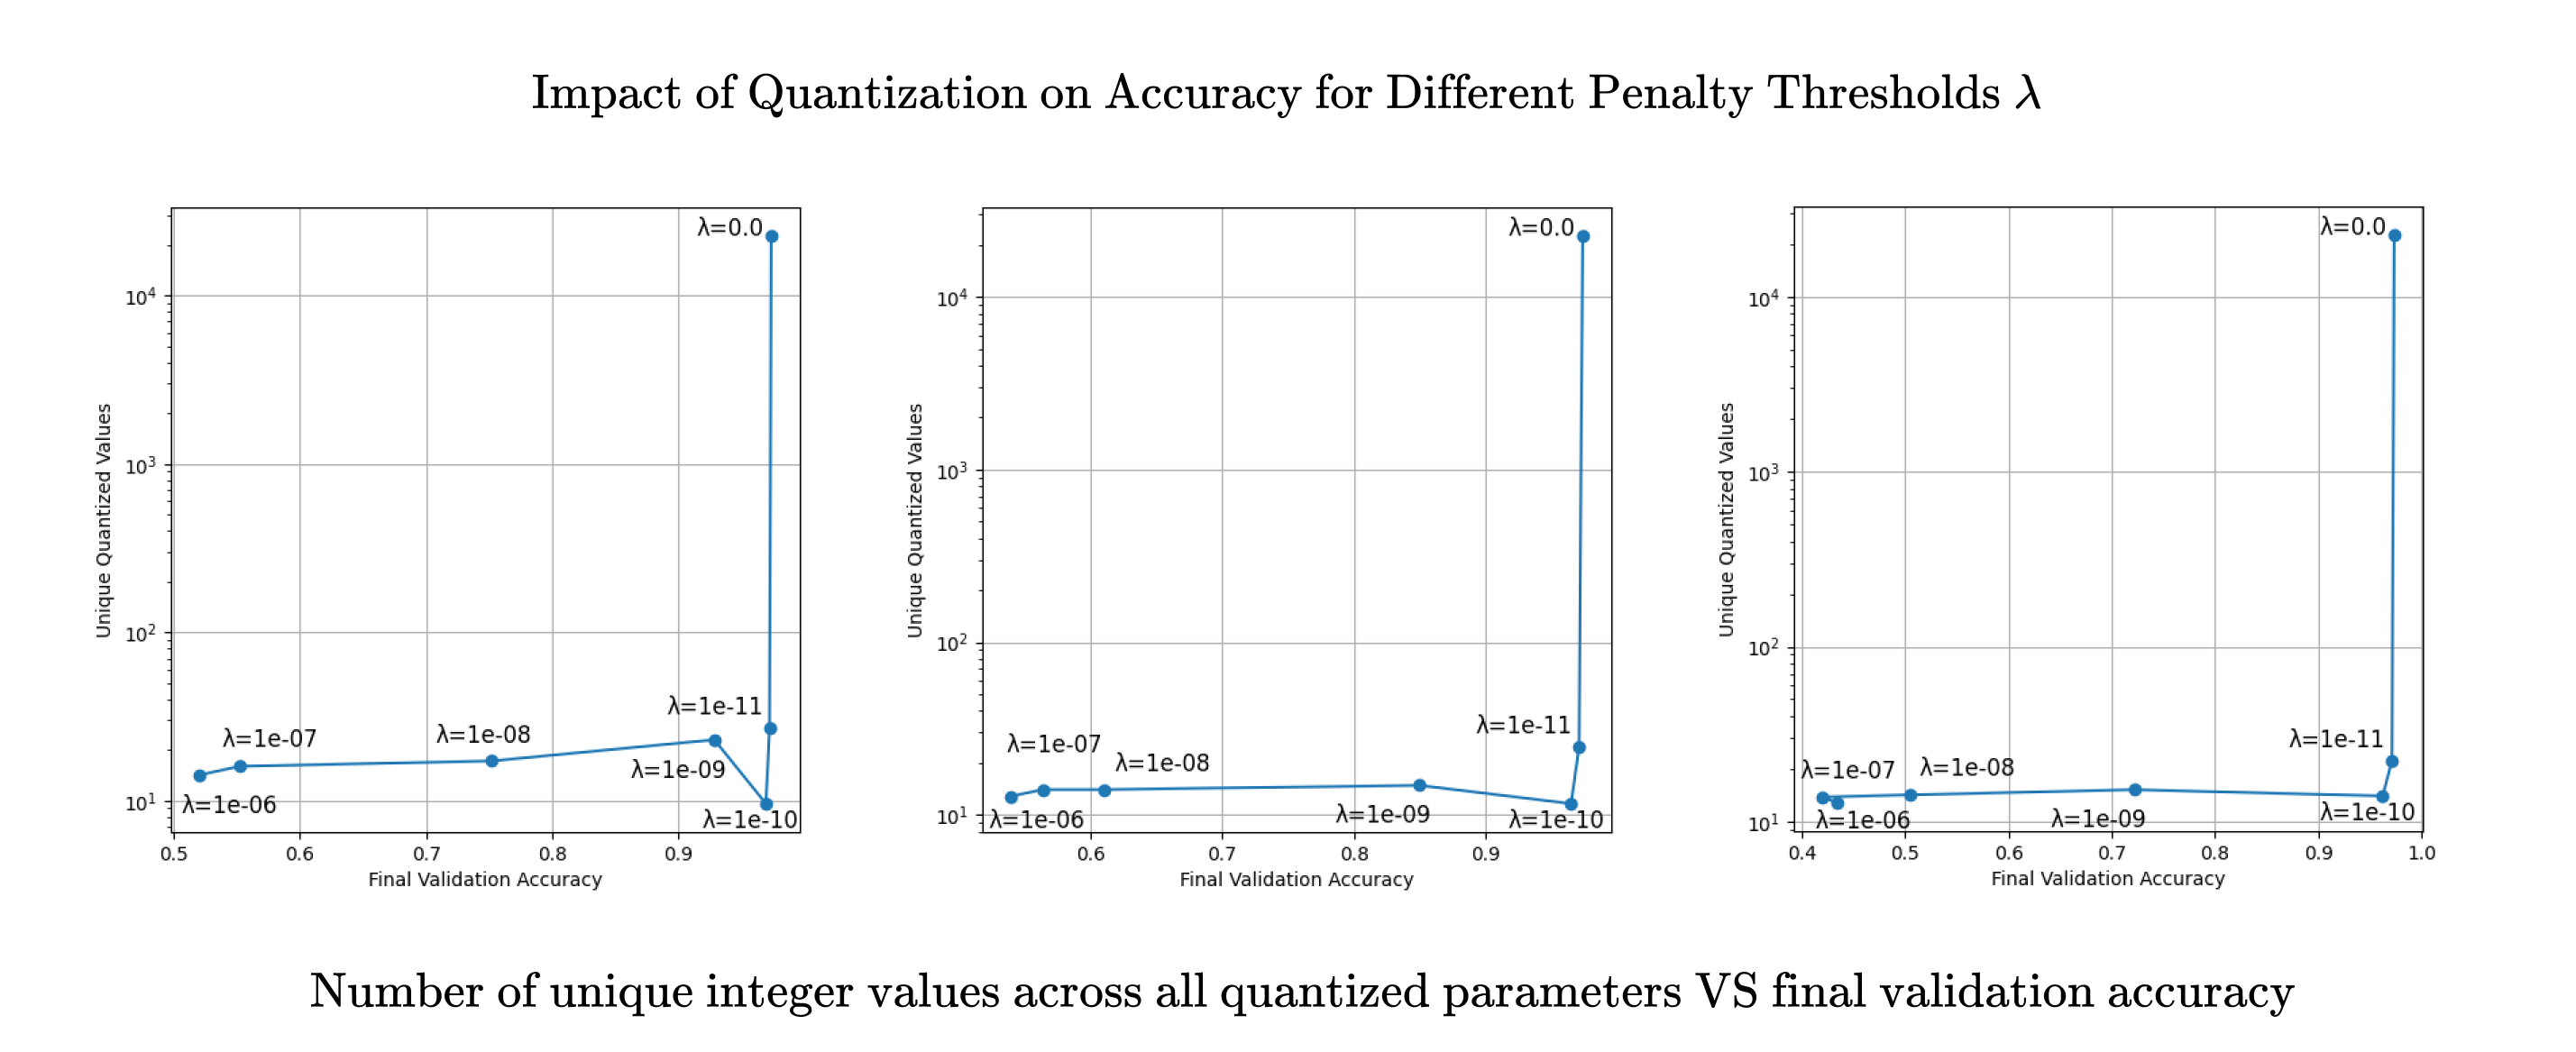
\includegraphics[width=14cm]{pareto-mnist-unique-vals-accuracy.png}
  \caption{Rowwise (left), columnwise (middle) and scalar (right) scaling factor applied to weights of dense layers, with a scalar scaling factor — to biases.
  We observe optimal quantization for \( \lambda = 10\)  in all cases. The values are averaged from the results of 5 training runs with different seeds.}
  \label{fig:pareto-mnist-unique-vals-accuracy}
\end{figure}


\begin{figure}[h!]
  \centering
  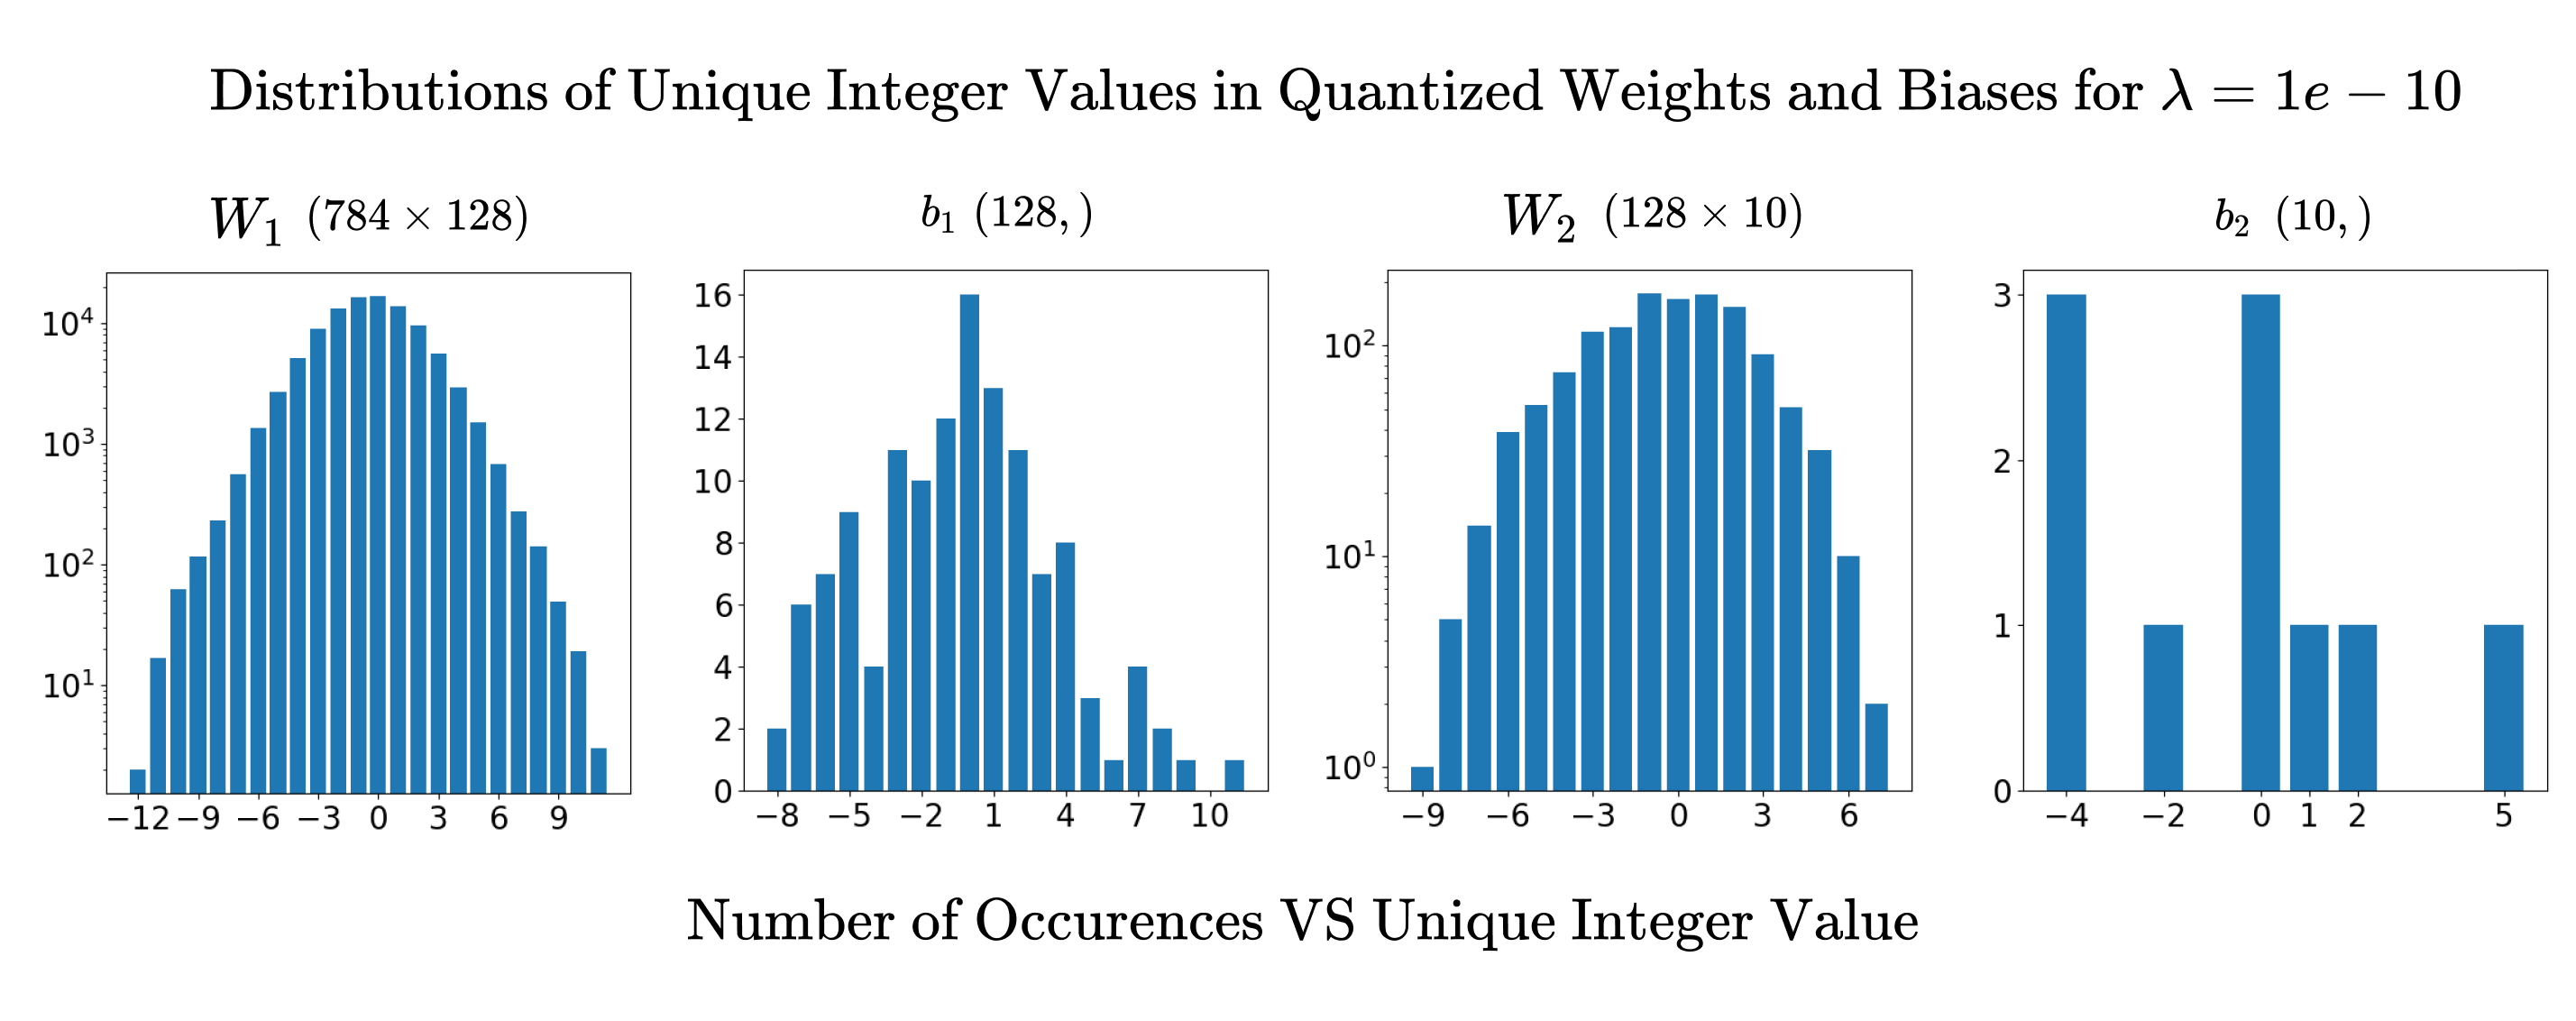
\includegraphics[width=14cm]{quantization_results_1e-10_dense.png}
  \caption{Rowwise scaling factors are applied to the weights of dense layers, while a scalar scaling factor is applied to the biases. Results are taken from the run with seed number 42.}
  \label{fig:quantization_results_1e-10_dense}
\end{figure}

\noindent There is, however, an interesting phenomenon to highlight. In all scenarios, 
when the penalty threshold becomes sufficiently large, the last parameter of the network,
\( b^2\) with shape (10,), begins to aggressively compensate for the quantization of the other parameters.
This observation is supported by the Pareto front plots in Figure \ref{fig:pareto-mnist-range-accuracy}, 
which, similar to Figure \ref{fig:pareto-mnist-unique-vals-accuracy}, illustrate the trade-off between accuracy and quantization.
However, instead of the number of unique values, they show the range of the final quantized integer values.
The increase in range as the penalty threshold increases is entirely attributable to the last bias vector. 
This behavior can be explained by the fact that, initially, 
when the other parameters are aggressively quantized, 
the last bias vector becomes critically important to the network and is less affected by quantization. 
However, when it eventually starts to undergo significant discretization, the model is already beyond repair.
\\
\\
Despite the behavior of the last bias vector, we consider this insignificant,
as biases are typically not quantized due to their limited contribution to the network's redundancy.
By the same token, it does not change the fact that the penalty threshold value of \( \lambda = 1e-10 \) still remains the optimum for dense layers,
as shown in Figure \ref{fig:val-accs-over-epochs-dense}, 
where validation accuracy stays nearly unchanged at \( \lambda = 1e-10 \),
while validation loss is within acceptable ranges from 
that of the baseline with no quantization as depicted in Figure \ref{fig:val-losses-over-epochs-dense}
 — all this despite the parameters being quantized to a range spanning from \( -5 \) to \( 5 \).
\\
\\
\begin{figure}[h!]
  \centering
  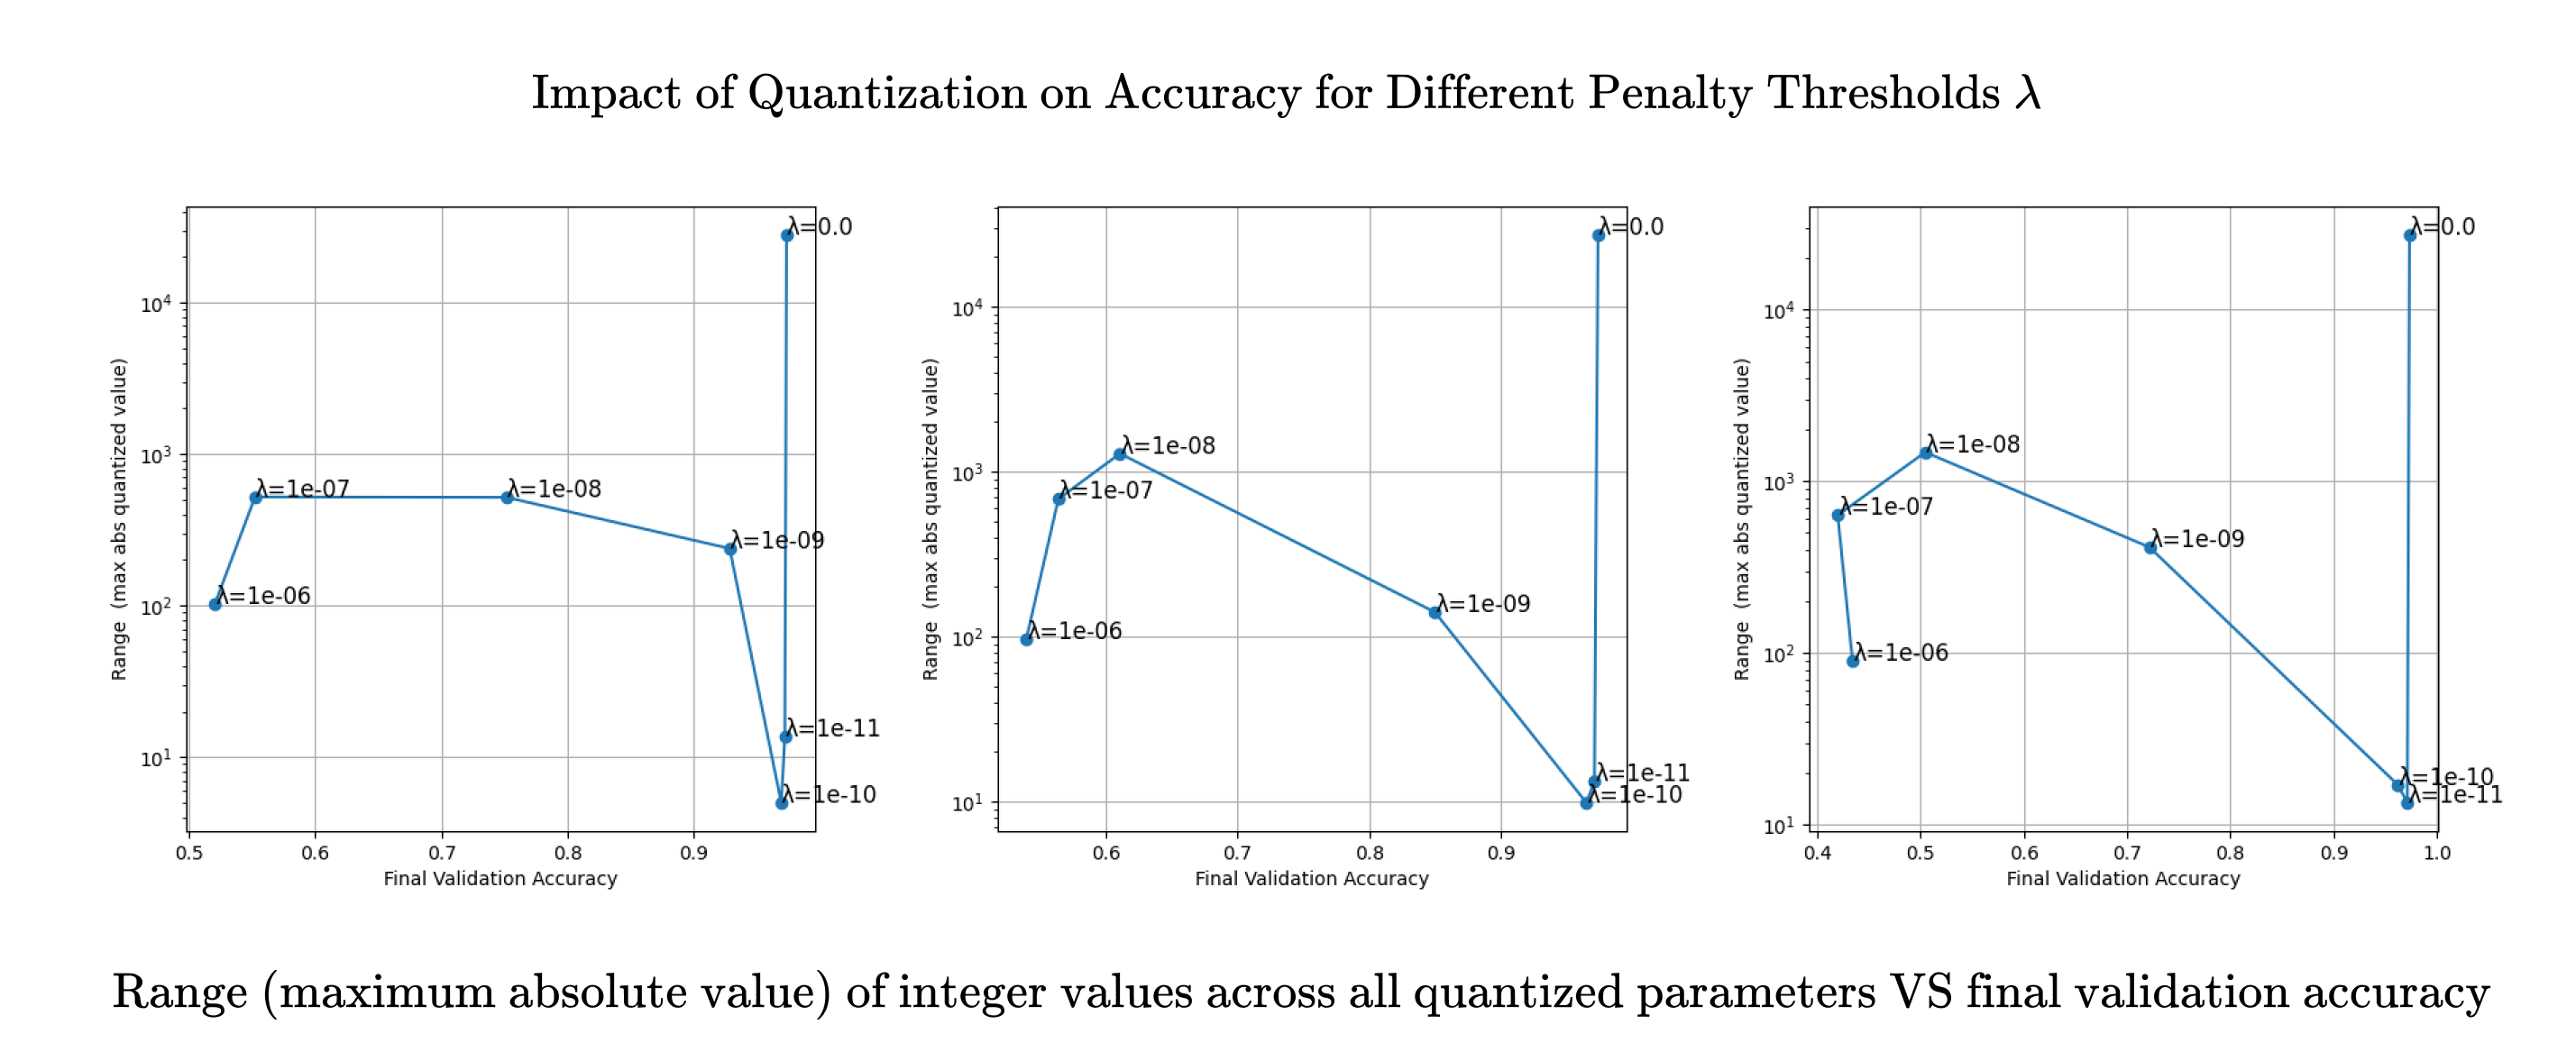
\includegraphics[width=14cm]{pareto-mnist-range-accuracy.png}
  \caption{Rowwise (left), columnwise (middle) and scalar (right) scaling factor applied to weights of dense layers, with a scalar scaling factor — to biases.  The values are averaged from the results of 5 training runs with different seeds.}
  \label{fig:pareto-mnist-range-accuracy}
\end{figure}
  
\begin{figure}[h!]
  \centering
  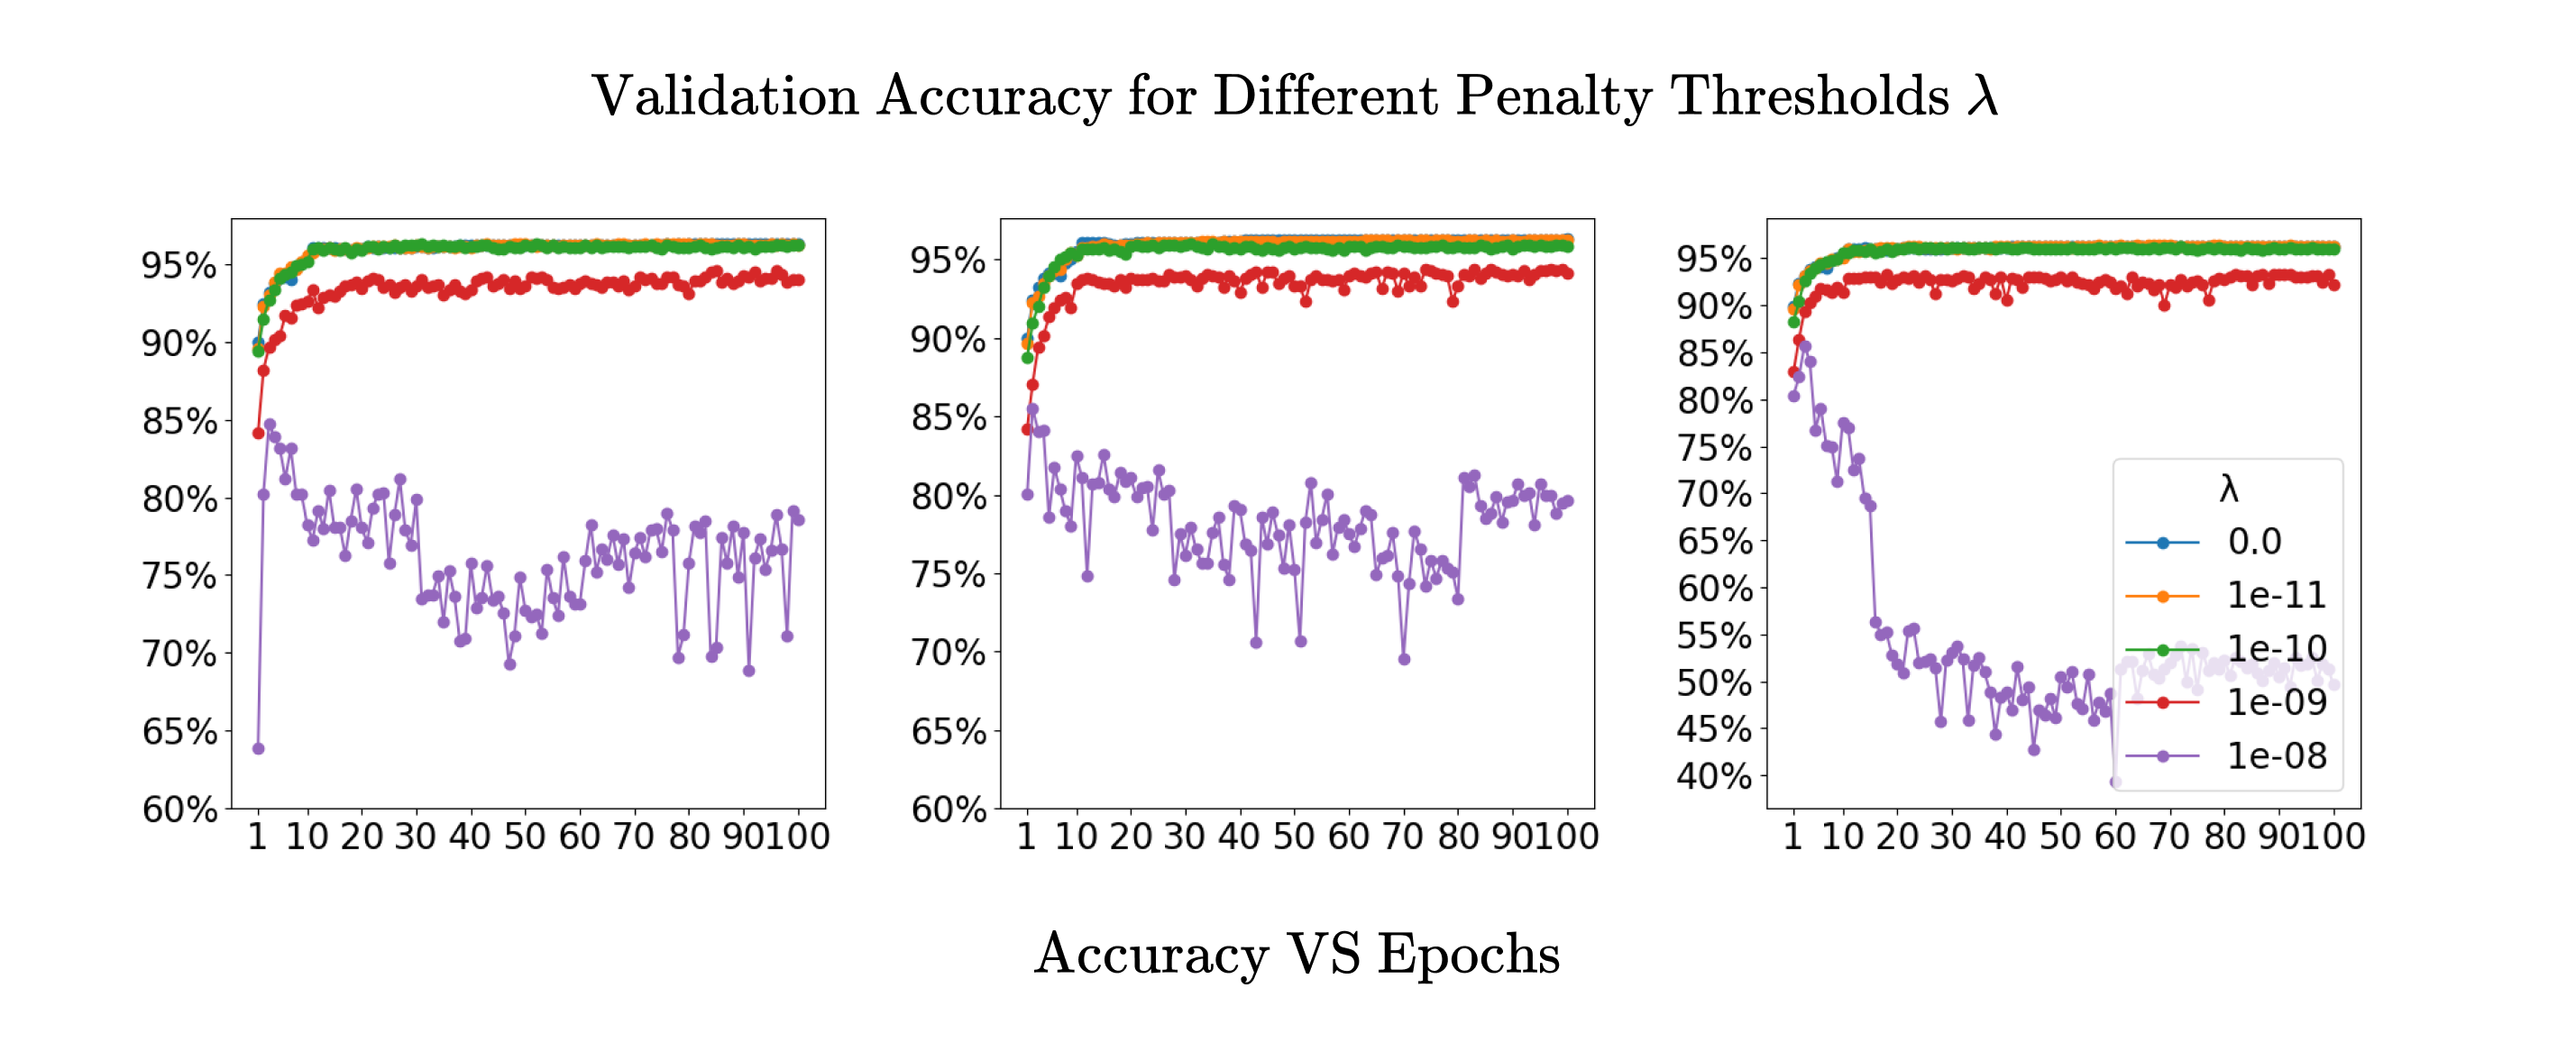
\includegraphics[width=14cm]{val-accs-over-epochs-dense.png}
  \caption{Rowwise (left), columnwise (middle) and scalar (right) scaling factor applied to weights of dense layers, with a scalar scaling factor — to biases. Results are taken from the run with seed number 42.}
  \label{fig:val-accs-over-epochs-dense}
\end{figure}

\begin{figure}[h!]
  \centering
  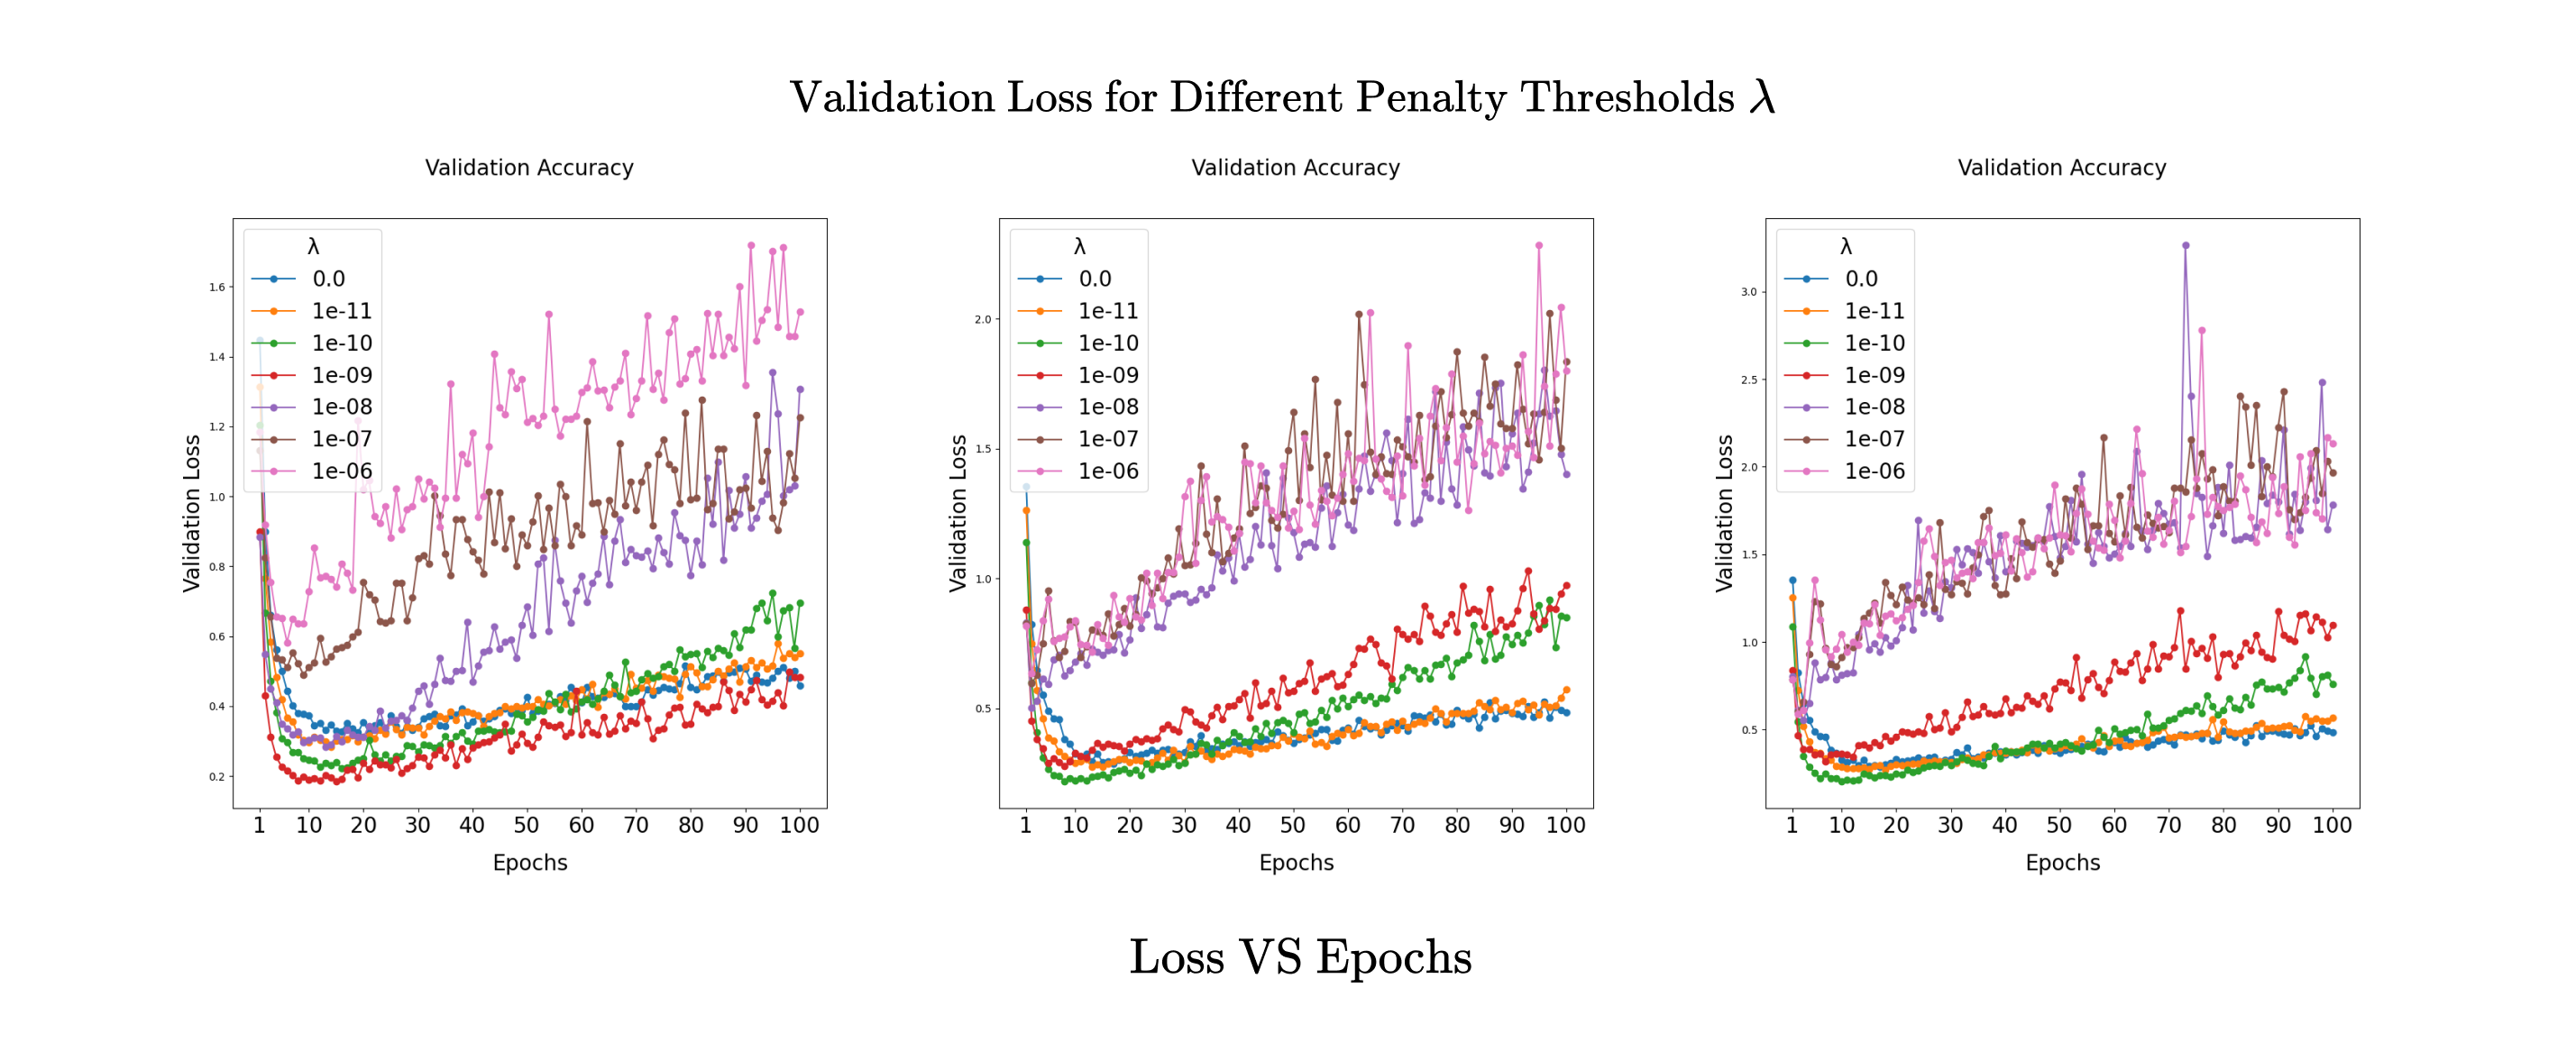
\includegraphics[width=14cm]{val-losses-over-epochs-dense.png}
  \caption{Rowwise (left), columnwise (middle) and scalar (right) scaling factor applied to weights of dense layers, with a scalar scaling factor — to biases. Results are taken from the run with seed number 42.}
  \label{fig:val-losses-over-epochs-dense}
\end{figure}
  
ADD THE RESULTS WHERE QUANTIZATION STARTS MID TRAINING
TO PROVIDE INFO FOR GRADUAL QUANTIZATION. TLDR: GUIDELINES FOR LAMBDA FOR GRADUAL 
QUANTIZATION

\subsection{Convolutional Layers}
\label{subsec:convolutionallayers}

\begin{figure}[h!]
  \centering
  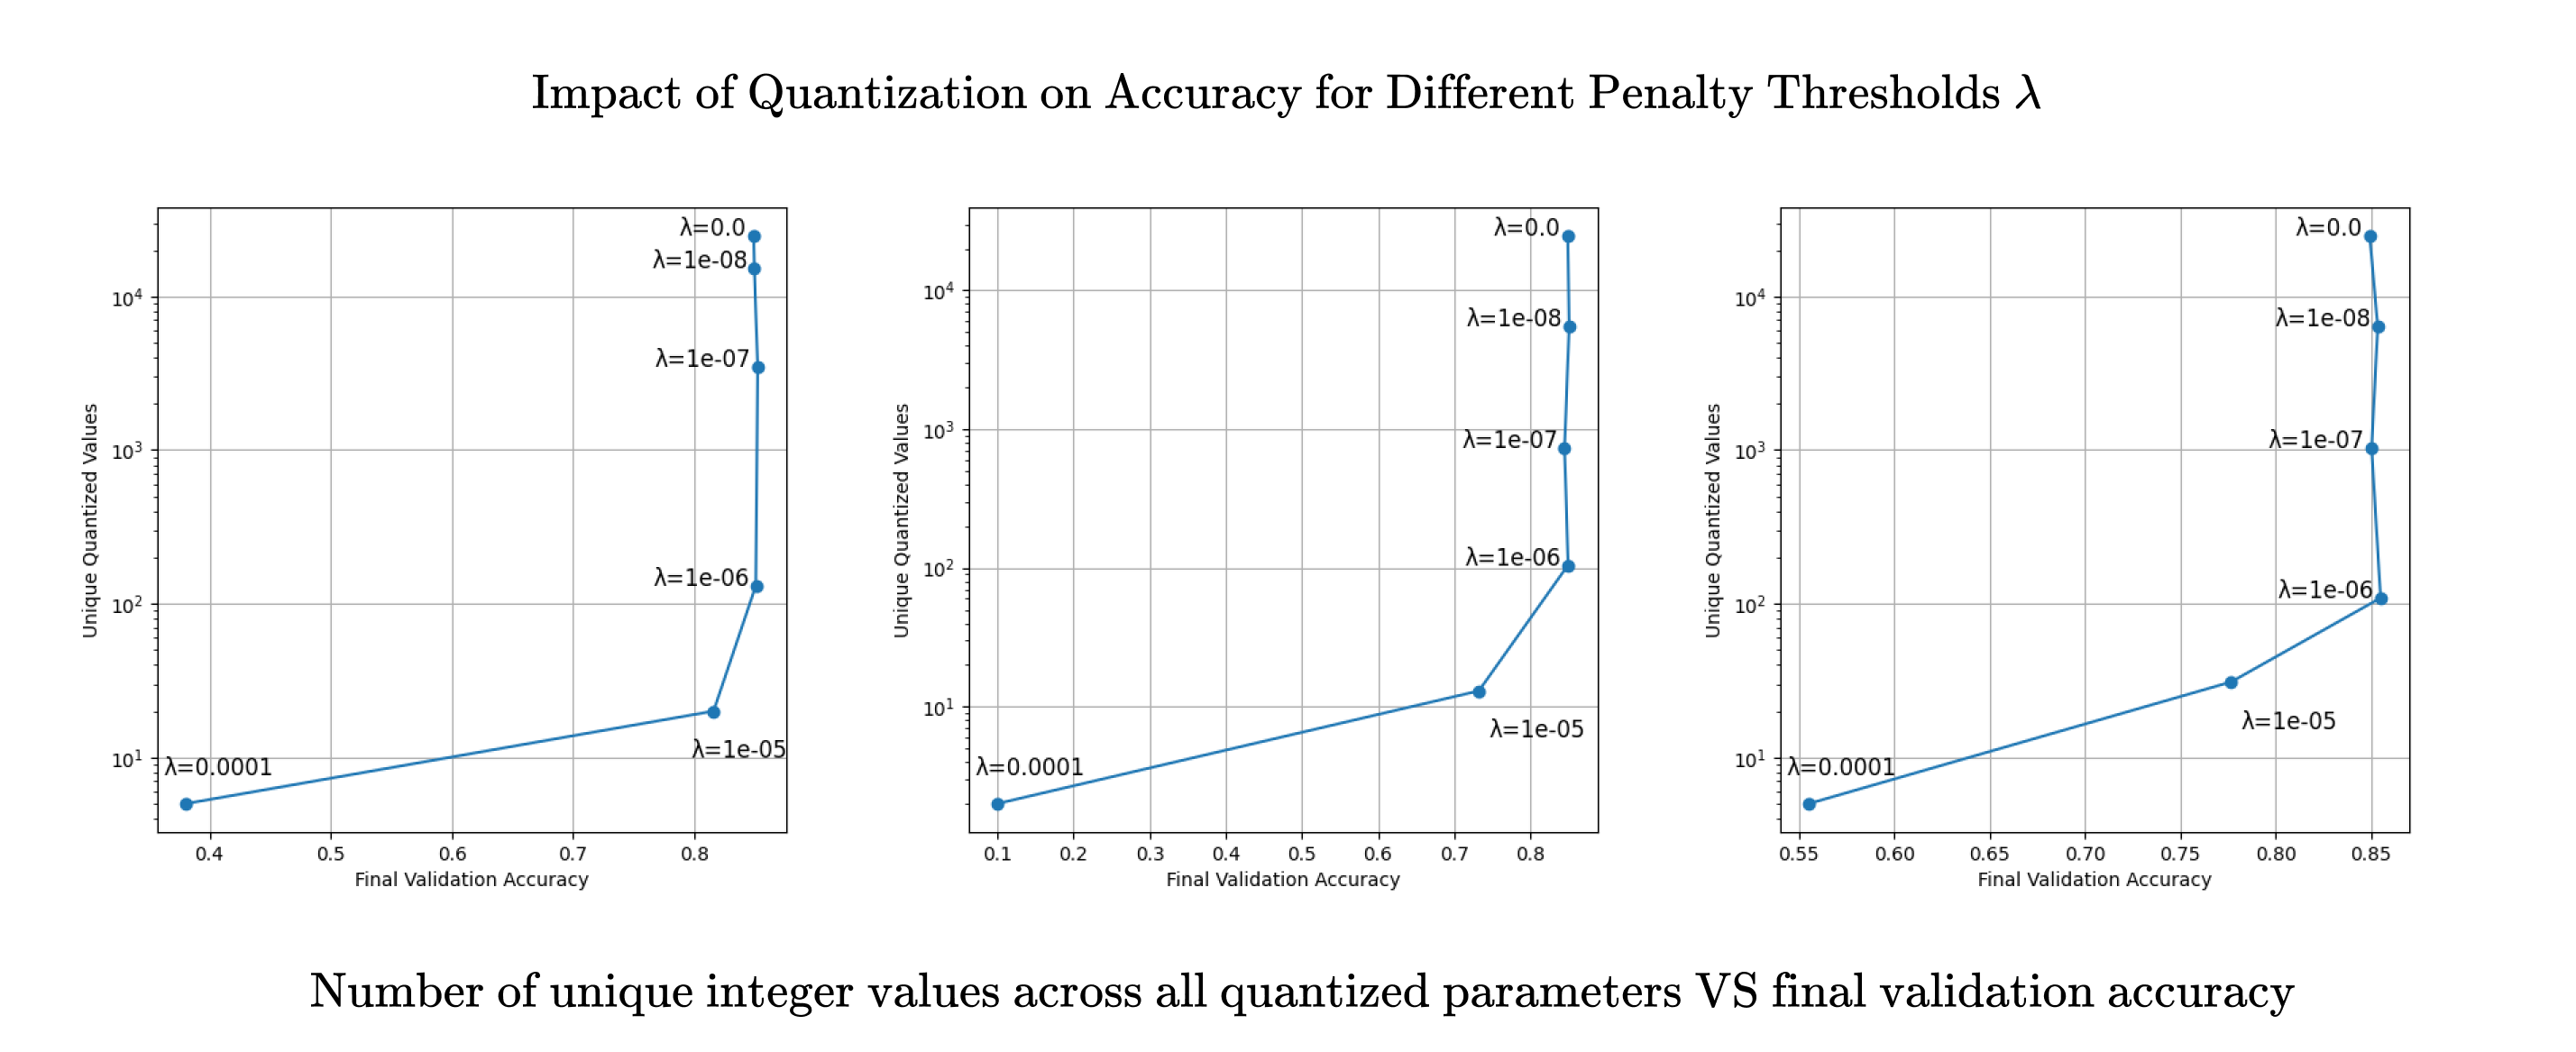
\includegraphics[width=14cm]{pareto-cifar-unique-vals-accuracy.png}
  \caption{Channelwise (left), rowwise (middle) and columnwise (right) scaling factor applied to kernels of convolutional layers, with a scalar scaling factor — to biases.
  We observe optimal quantization for \( \lambda = 10\)  in all cases. The values are averaged from the results of 5 training runs with different seeds.}
  \label{fig:pareto-mnist-unique-vals-accuracy}
\end{figure}

\begin{figure}[h!]
  \centering
  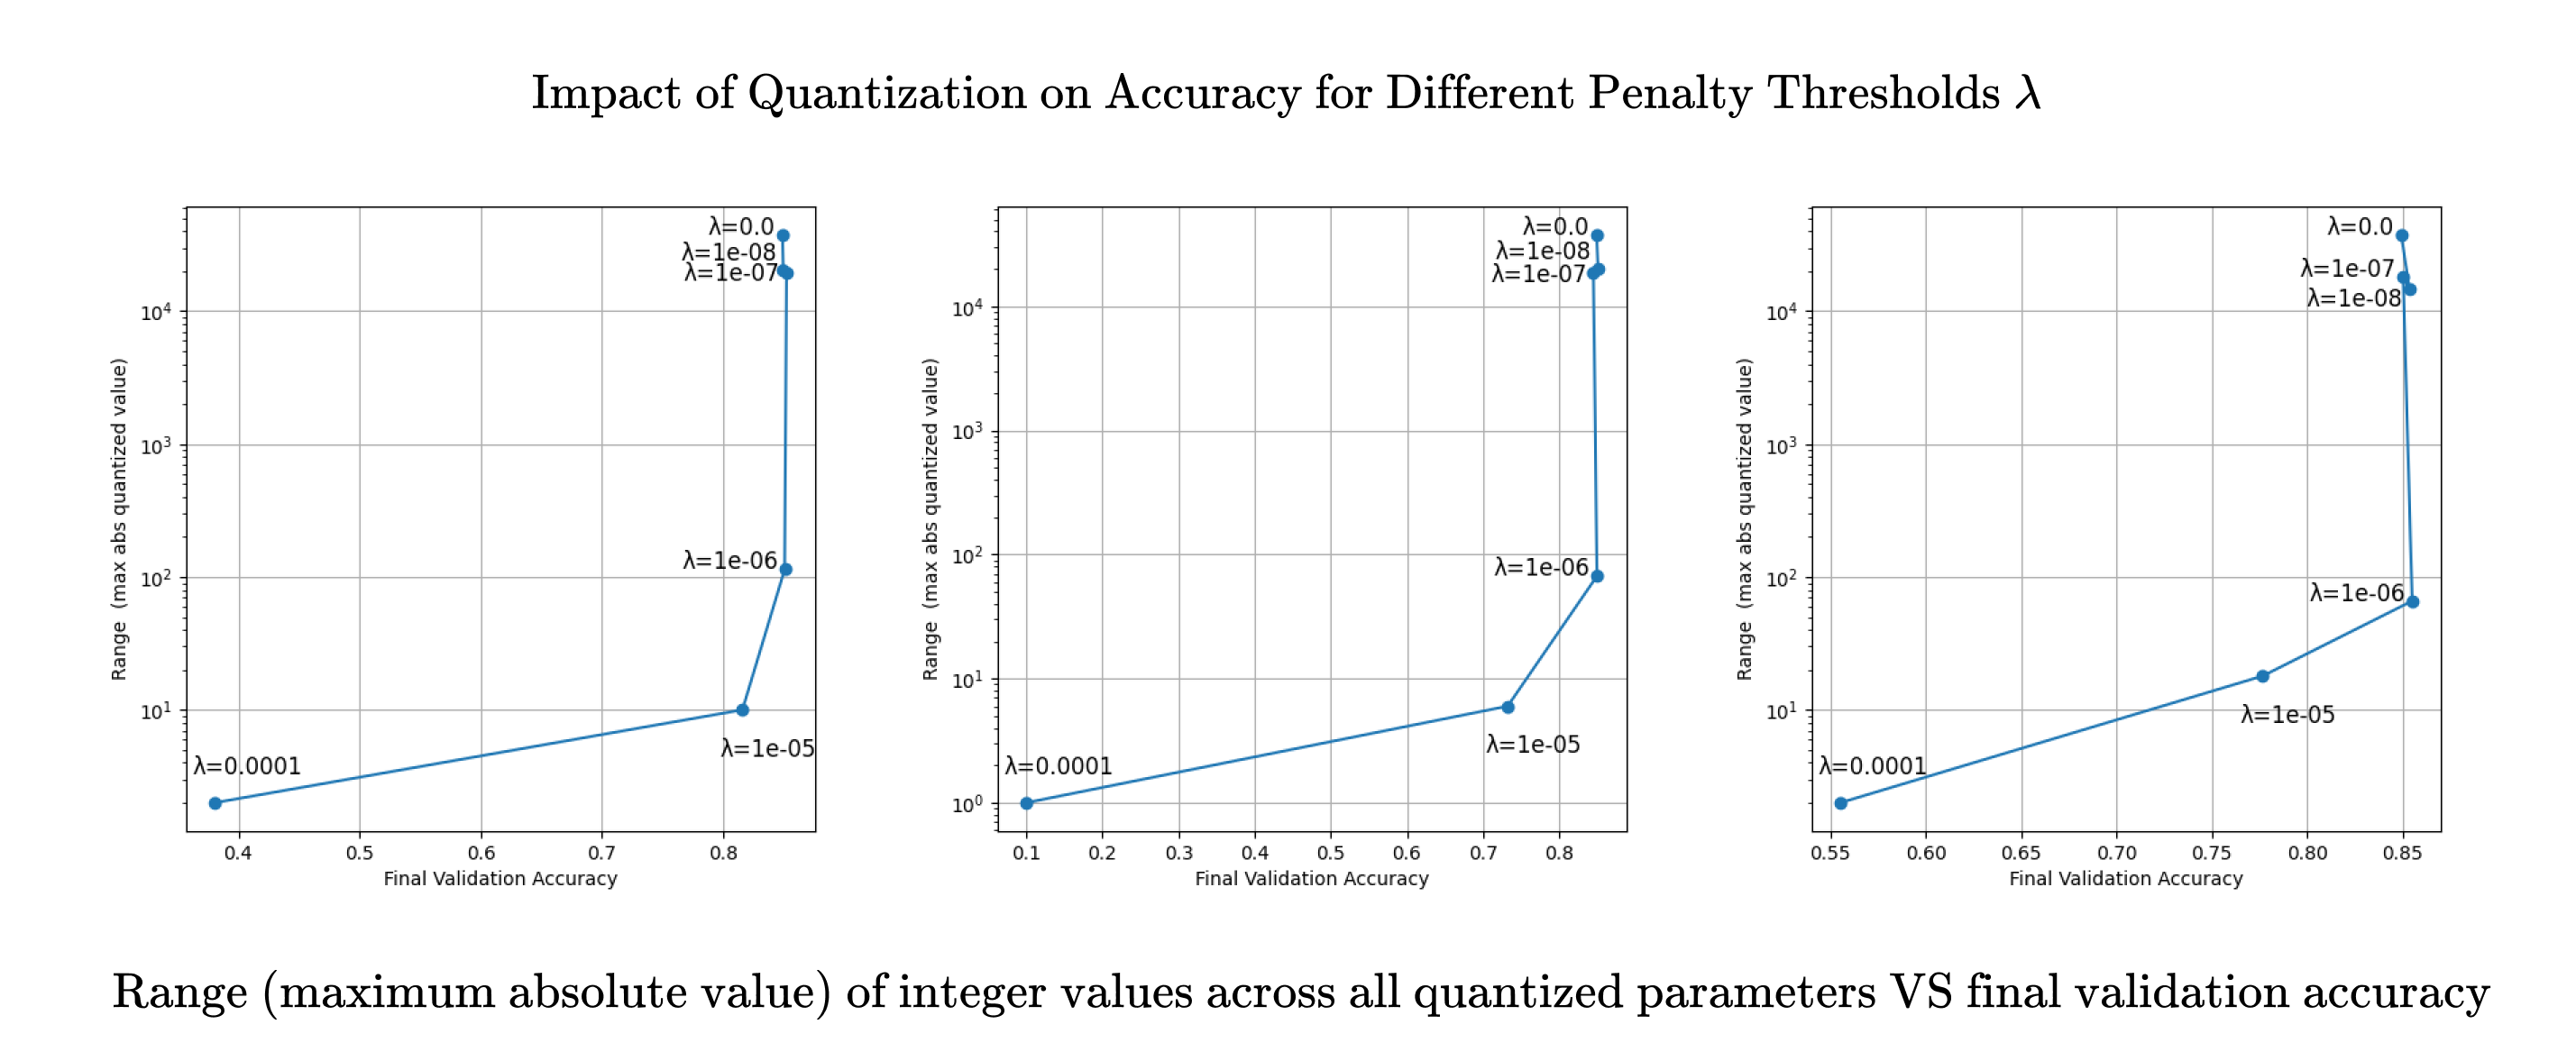
\includegraphics[width=14cm]{pareto-cifar-range-accuracy.png}
  \caption{Channelwise (left), rowwise (middle) and columnwise (right) scaling factor applied to kernels of convolutional layers, with a scalar scaling factor — to biases.  The values are averaged from the results of 5 training runs with different seeds.}
  \label{fig:pareto-mnist-range-accuracy}
\end{figure}

\begin{figure}[h!]
  \centering
  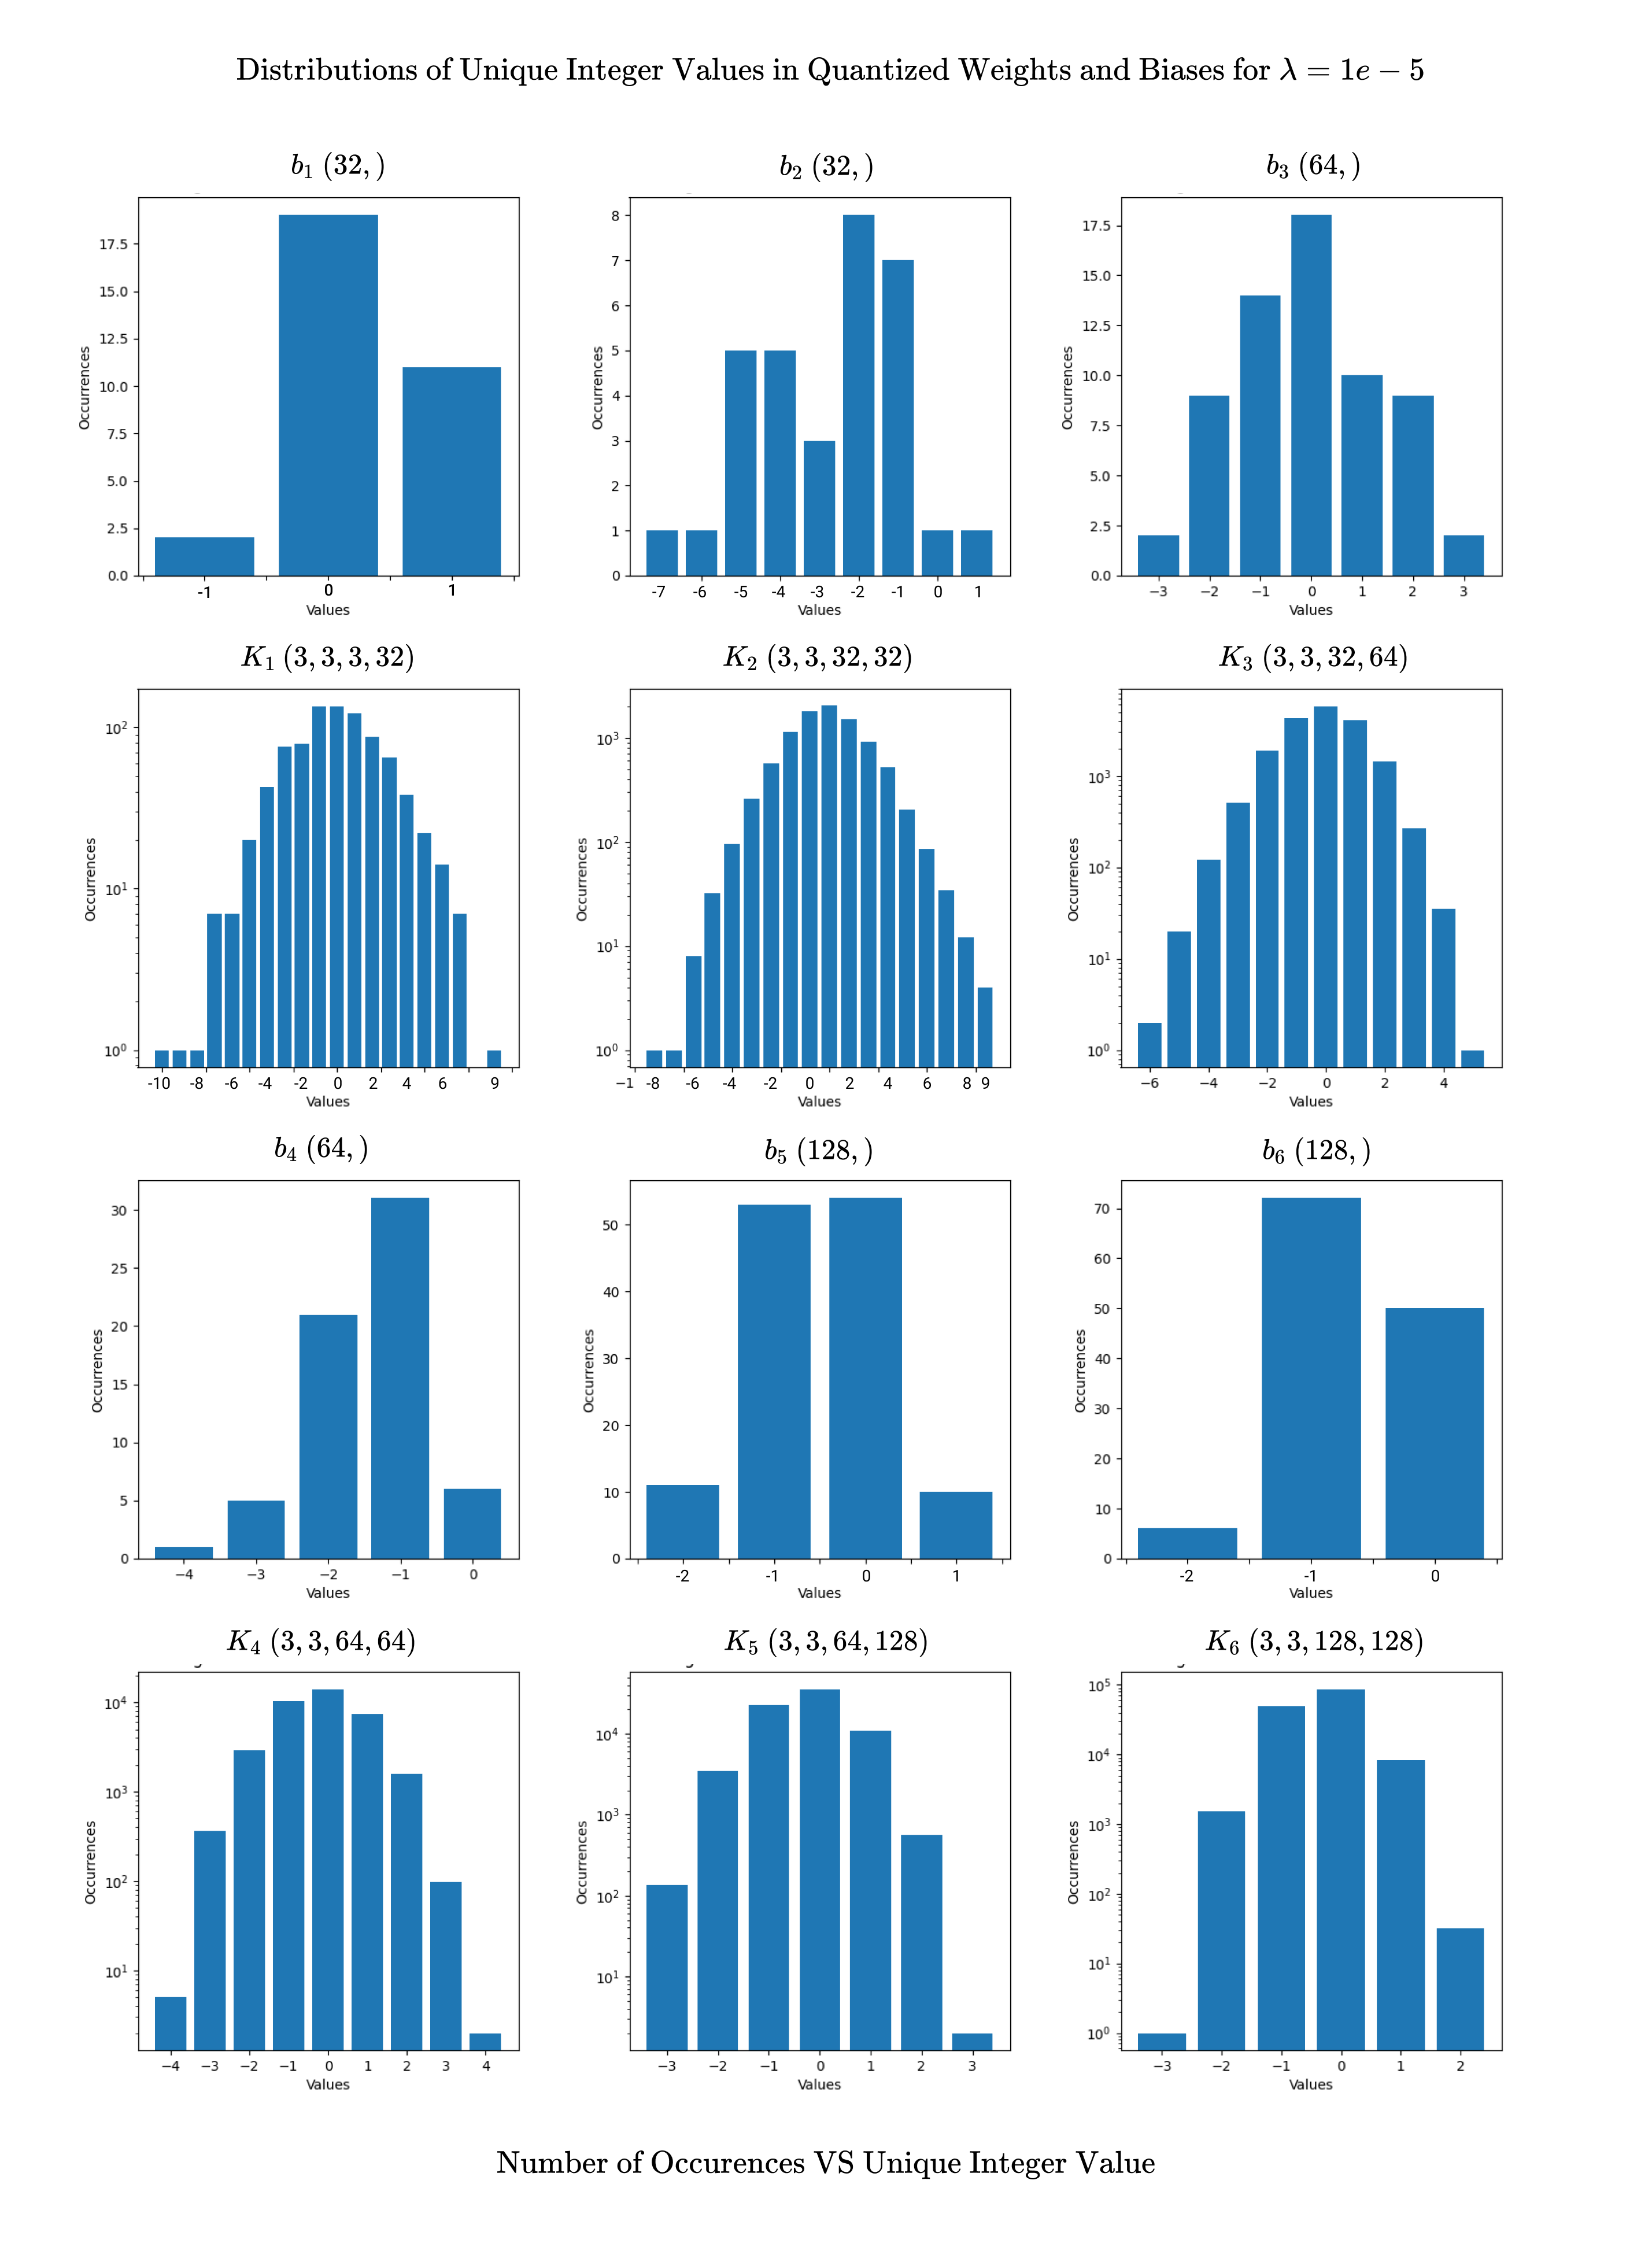
\includegraphics[width=15cm]{quantization_results_1e-5_conv.png}
  \caption{Channelwise scaling factors are applied to the kernels of convolutional layers, while a scalar scaling factor is applied to the biases. Results are taken from the run with seed number 42.}
  \label{fig:quantization_results_1e-10_dense}
\end{figure}

\begin{figure}[h!]
  \centering
  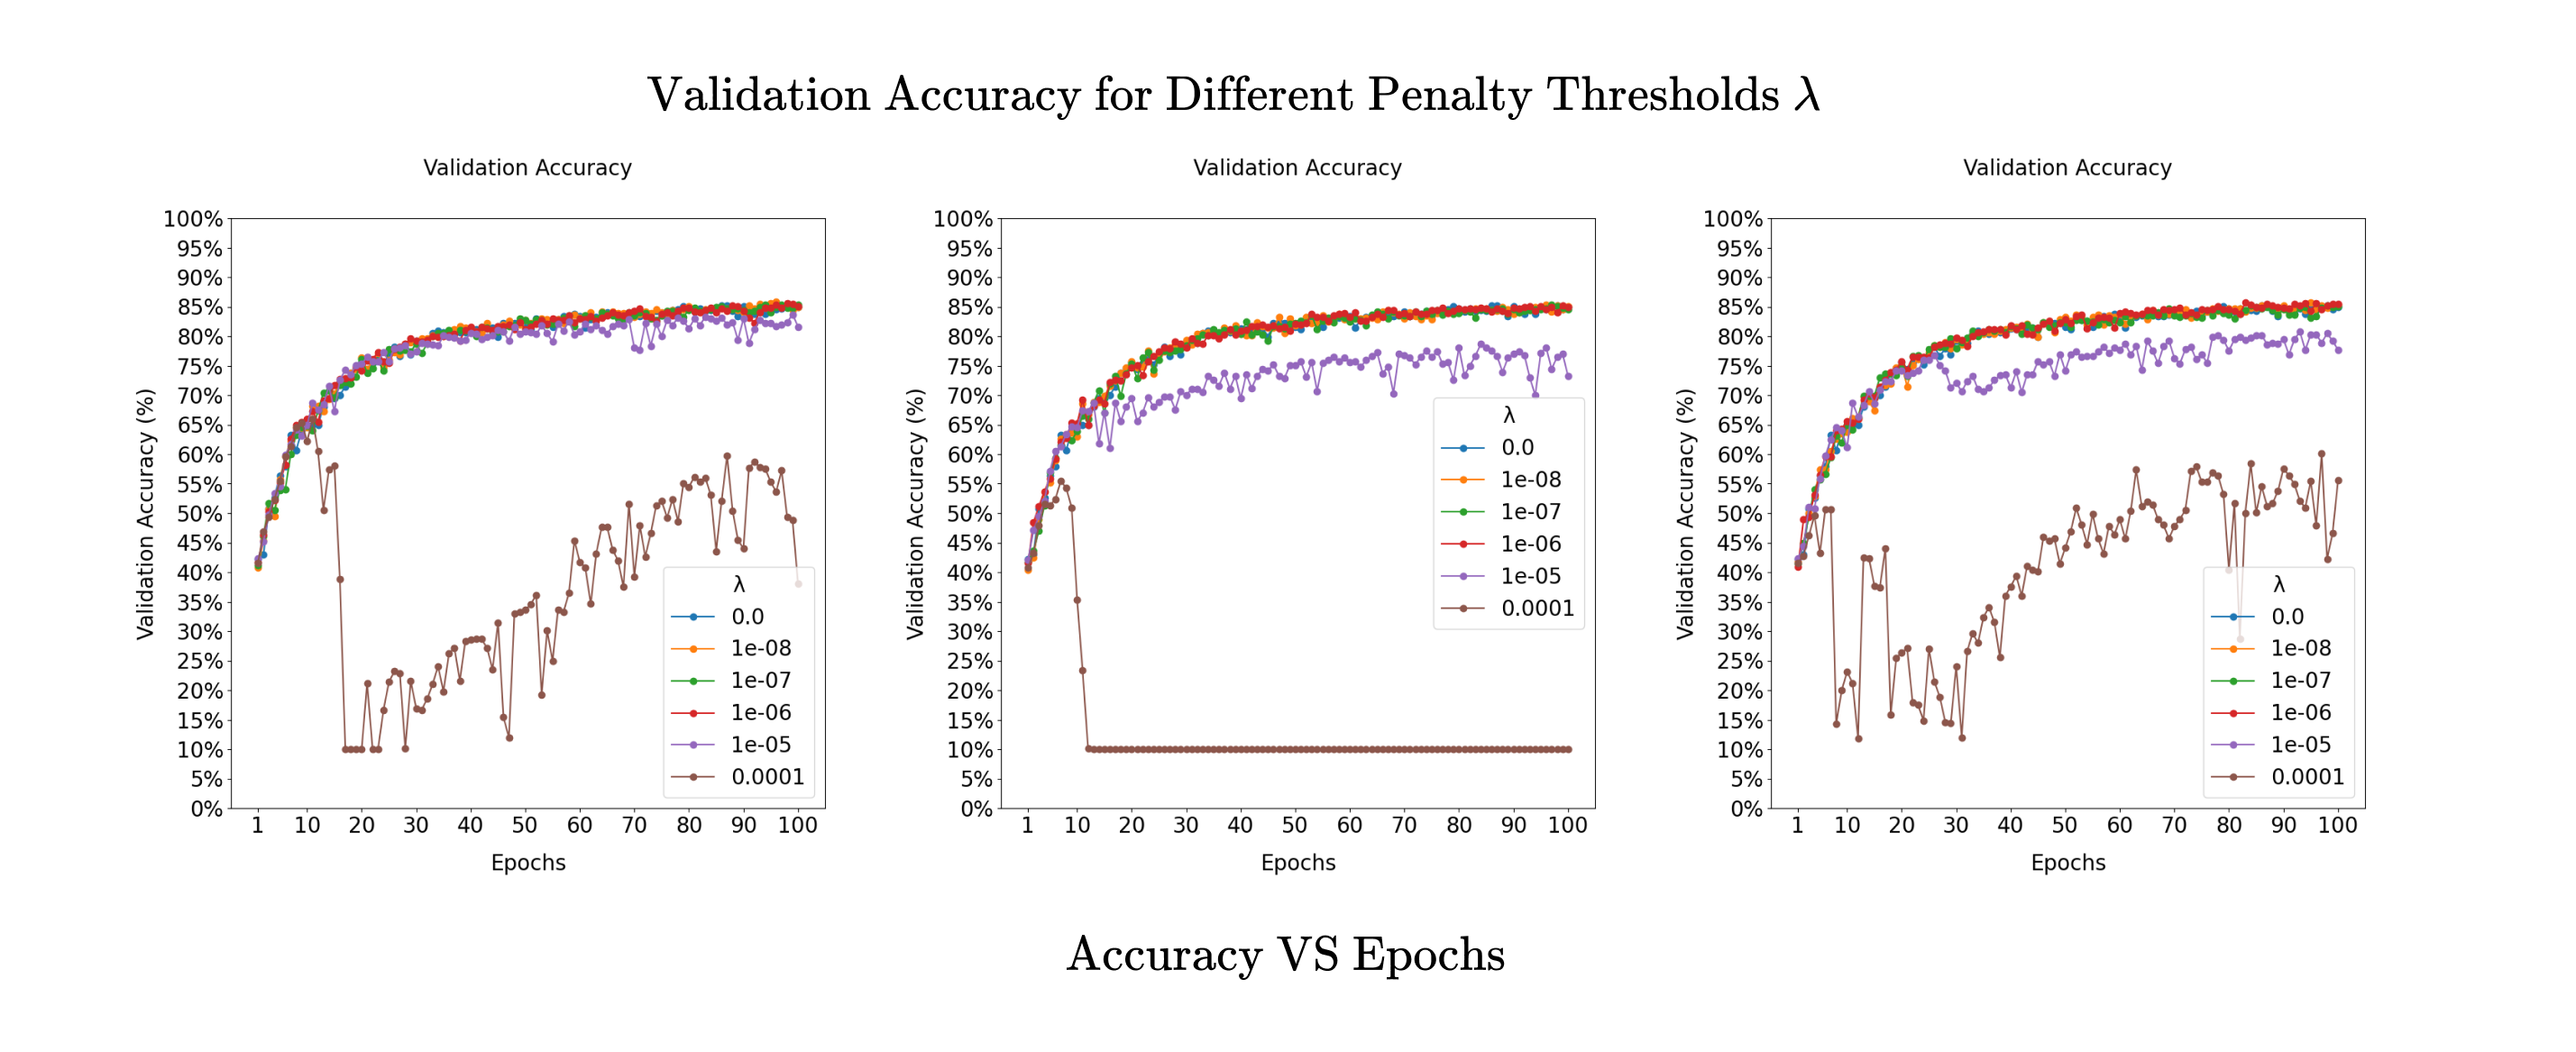
\includegraphics[width=14cm]{val-accs-over-epochs-conv.png}
  \caption{Channelwise (left), rowwise (middle) and columnwise (right) scaling factor applied to kernels of dense layers, with a scalar scaling factor — to biases. Results are taken from the run with seed number 42.}
  \label{fig:val-accs-over-epochs-dense}
\end{figure}

\begin{figure}[h!]
  \centering
  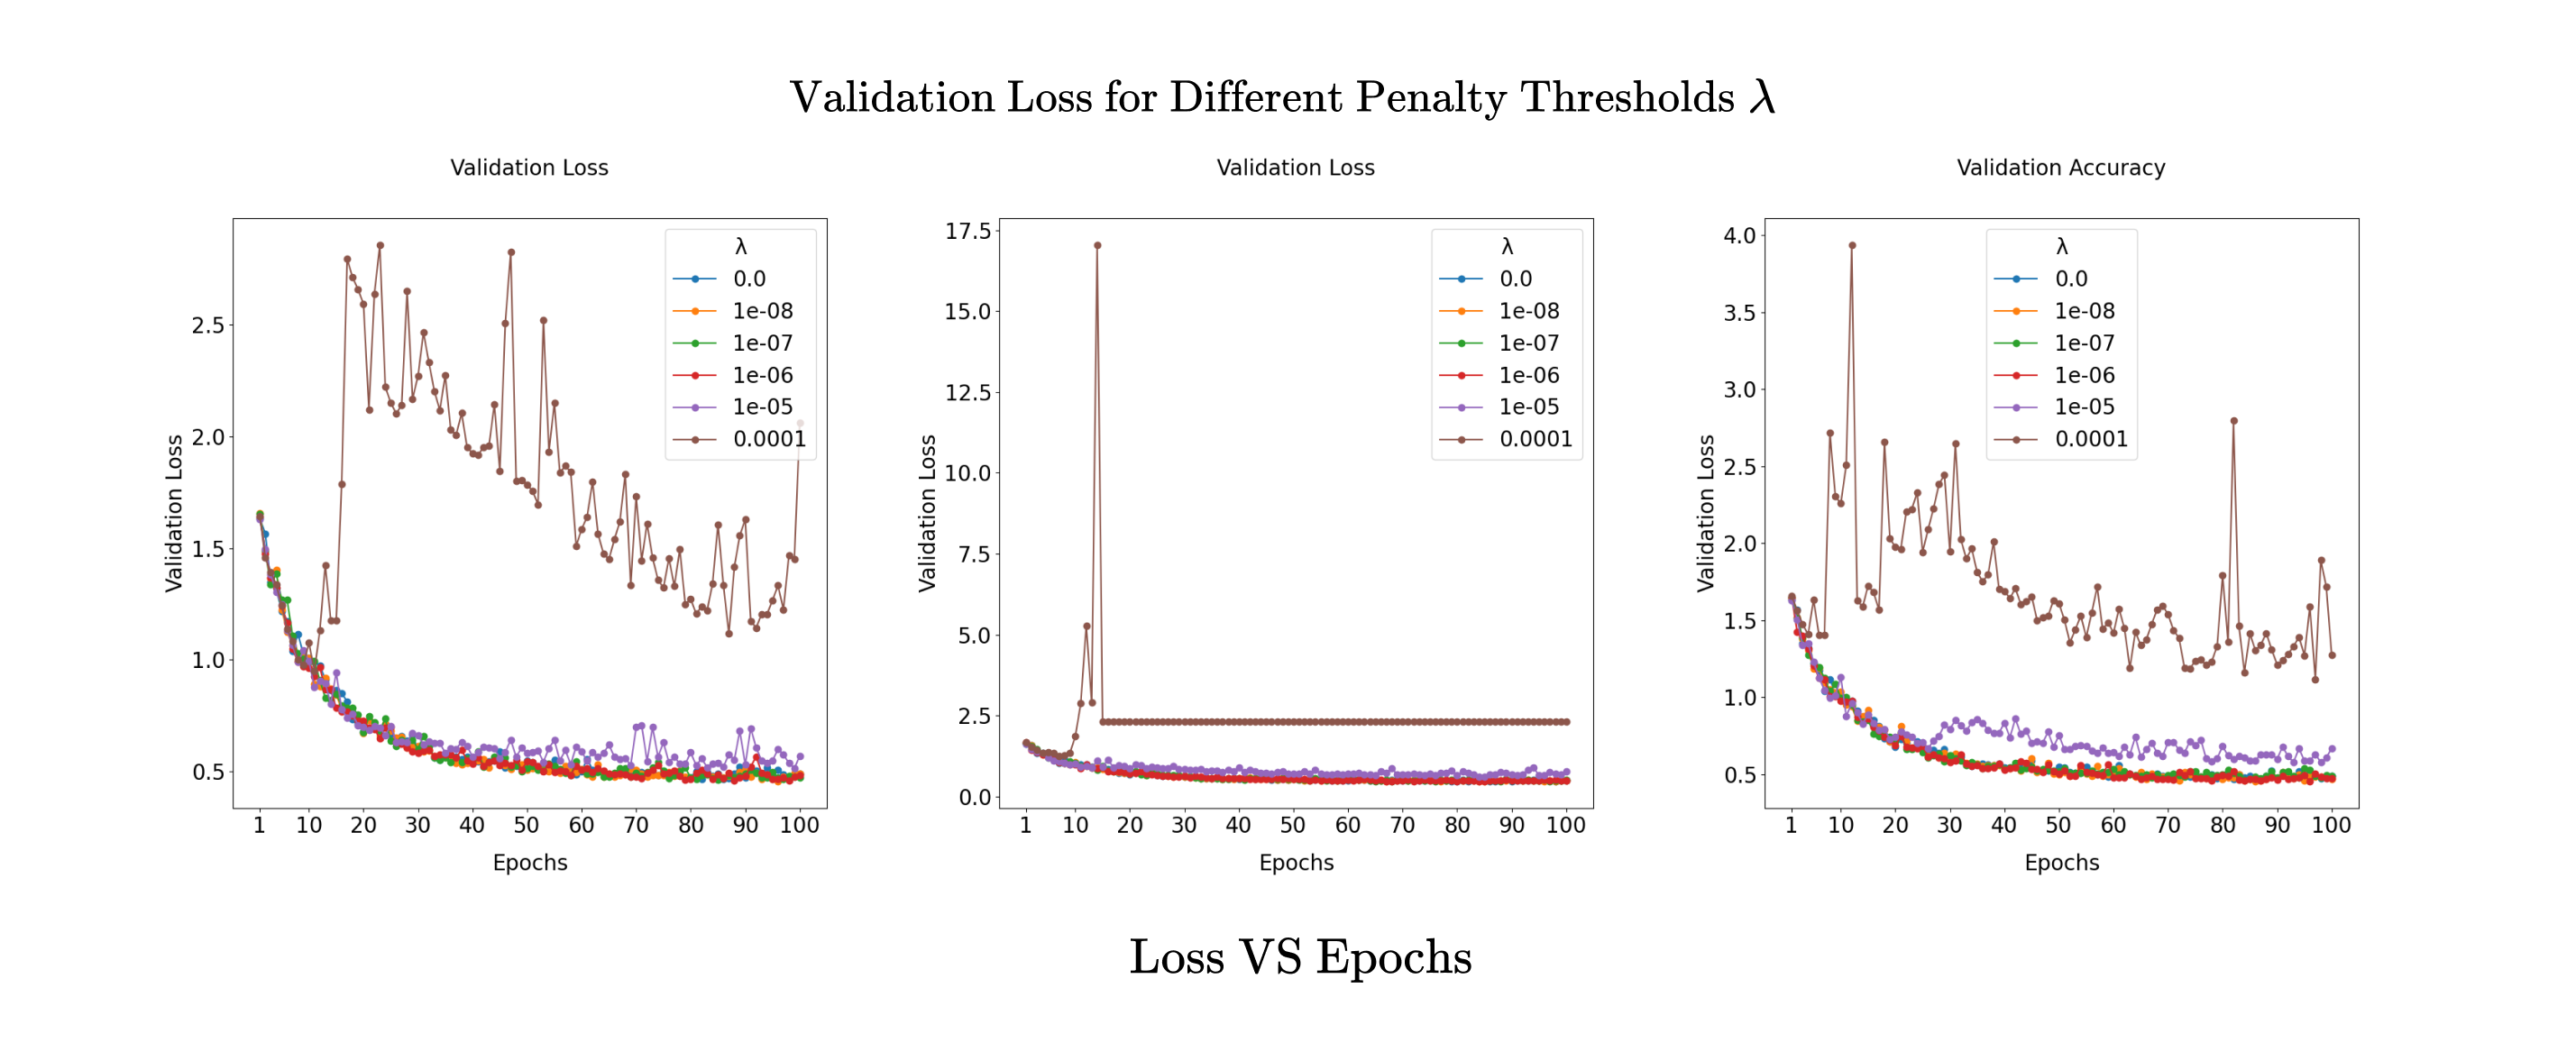
\includegraphics[width=14cm]{val-losses-over-epochs-conv.png}
  \caption{Channelwise (left), rowwise (middle) and columnwiselar (right) scaling factor applied to kernels of dense layers, with a scalar scaling factor — to biases. Results are taken from the run with seed number 42.}
  \label{fig:val-losses-over-epochs-dense}
\end{figure}
% ------------------------------------------------------------
% ----------------------- Custom loss terms analysis ----------------------- 
% ------------------------------------------------------------

\section{Systematic Analysis of Custom Loss Terms}
\label{sec:dataset}

